\chapter{Analysis and Design}

This chapter will firstly provide an overview of ROS and the condition of YuMi robot that affects the design choices. The next two sections will then present the system design overview and detailed system workflow respectively.

\section{ROS and YuMi Overview}
As discussed in the Background Chapter, ROS handles a number of independent Nodes that performs specific function(s). They communicate with each other by publishing messages to topics or subscribing them. ROS messages support several data formats, including number, string, and time etc. Moreover, these communications are only available if a $roscore$ is running, which is a collection of programs and Nodes that are prerequisites of a ROS-based system. Besides, $TF$ is an important package in ROS and used several times in this project. According to \citep{tfROSWik}, it maintains the relationship between coordinate frames (such as camera frame, robot frame etc.) in a tree structure buffered, which enables the user to transform points, vectors, etc between any two coordinate frames at any desired point in time. Details will be discussed in Implementation Chapters.

The dual-arm robot YuMi communicates with ROS using the Personal Robotics Lab setup (see User Guide Chapter for more details). YuMi has one gripper camera embedded in each of its grippers. Using these cameras may provide more accurate results of shoe and shoe hole locations (more discussion in Future Work Section \ref{futurecamera}). However, in order to use these two cameras, a package named $abb\_rws\_interface$ which is a proprietary interface of ABB is required. According to \citep{EGMfiles}, it is not public. Also, the open source version of that package called $abb\_librws$ cannot match the current $yumi\_cameras$ setup. Furthermore, it is not very feasible to tie a small camera to YuMi's arms because the available movement range will be limited. Therefore, this project will only utilize the ASUS Xtion or ZED Mini camera for detection.

\section{System Overview}

\begin{figure}[H]
\centering
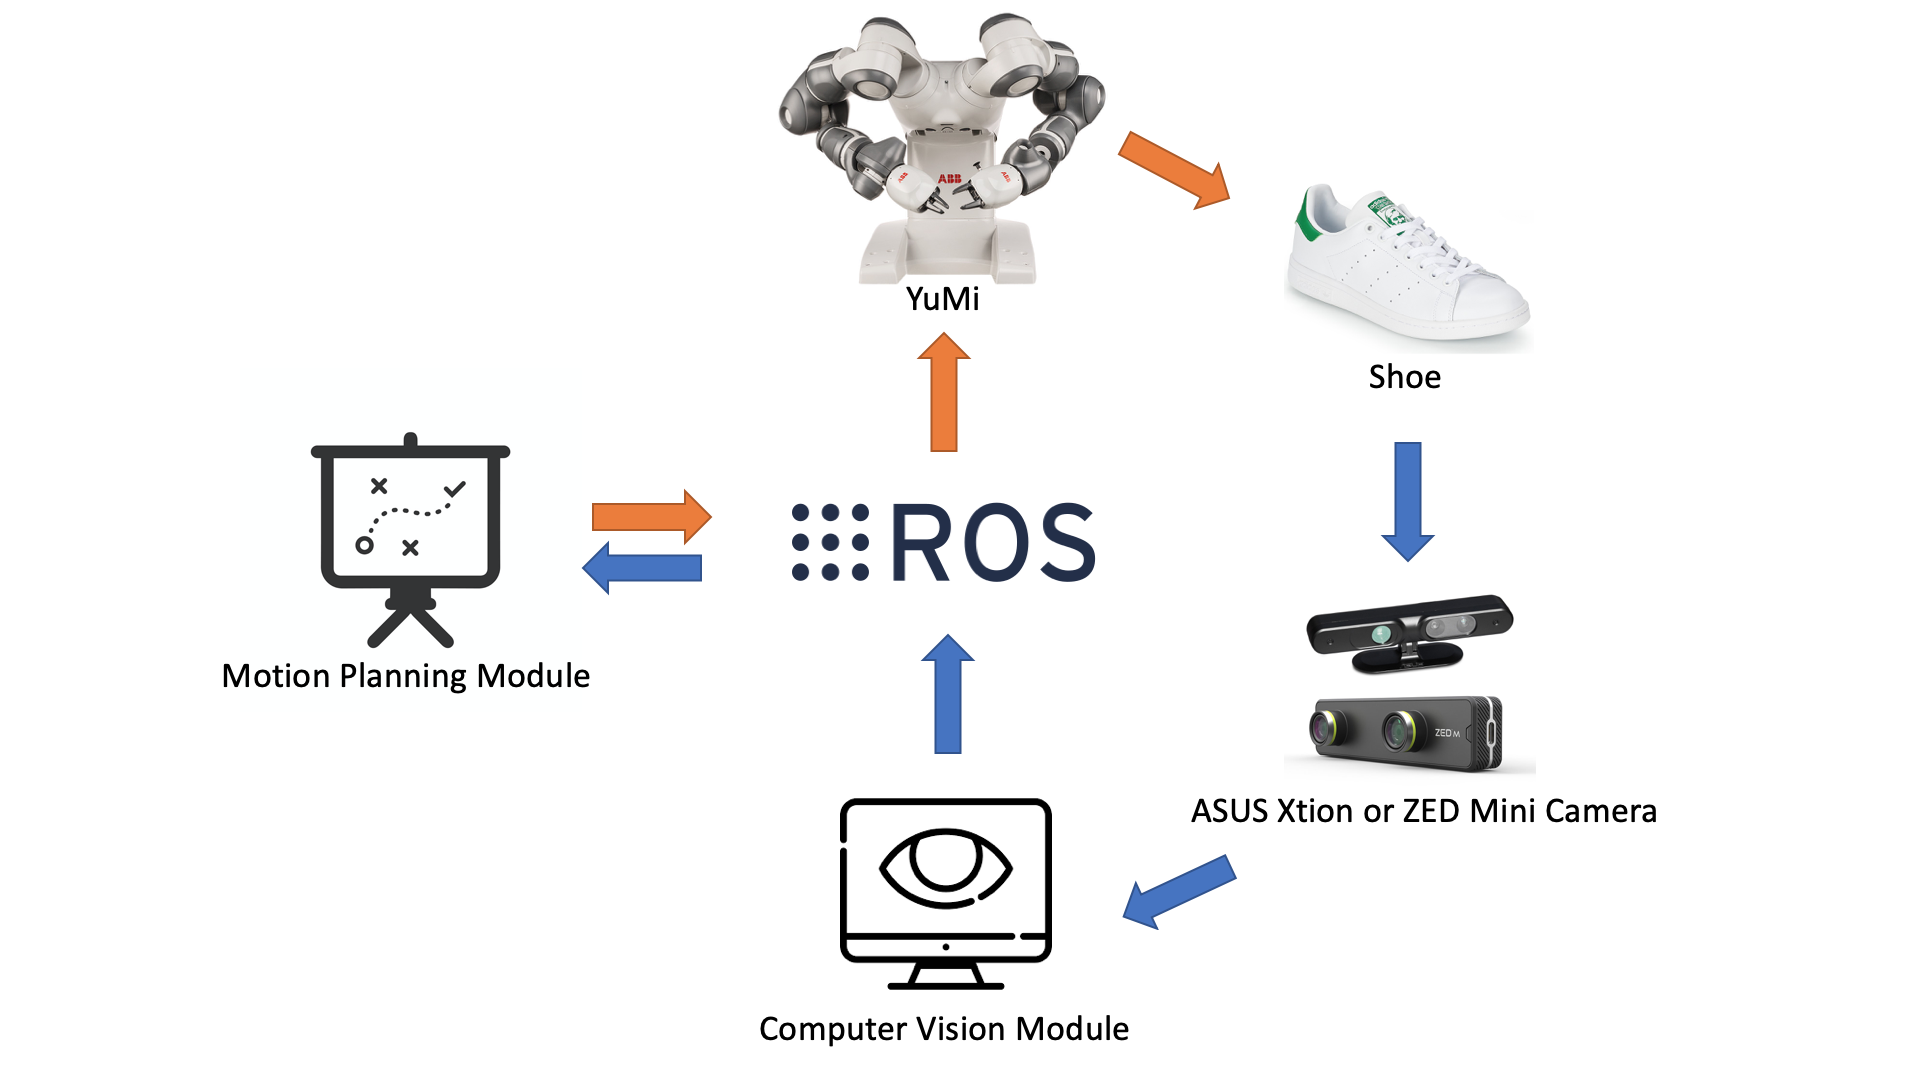
\includegraphics[width = \columnwidth]{AnalysisDesign/system.png}
\caption{An overview of the designed system. Blue arrows represent computer vision messages, and orange arrows indicate related motion plans and manipulations.}
\label{c4}
\end{figure}

Figure \ref{c4} displays the system overview of this project, which consists of six components: the shoe, the camera, computer vision module, ROS Kinetic, motion planning module, and YuMi. Starting from the camera, which consistently recording RGB and depth images of the workbench and outputs them to the computer vision module. The module then performs several functions including shoe detection, shoe hole tracking, 6D shoe hole pose estimation etc and publishes the corresponding messages to ROS several topics. After that, the motion planning module subscribes this information and plans YuMi arms trajectories accordingly to adjust shoe pose or put shoelace on a hole, etc. If the planning succeeds, YuMi will then execute these motions for real manipulations. The cycle then goes back to the beginning, and the camera keeps providing information to computer vision module.

%detail---------------------------
\section{System Workflow}

\begin{figure}[H]
\centering
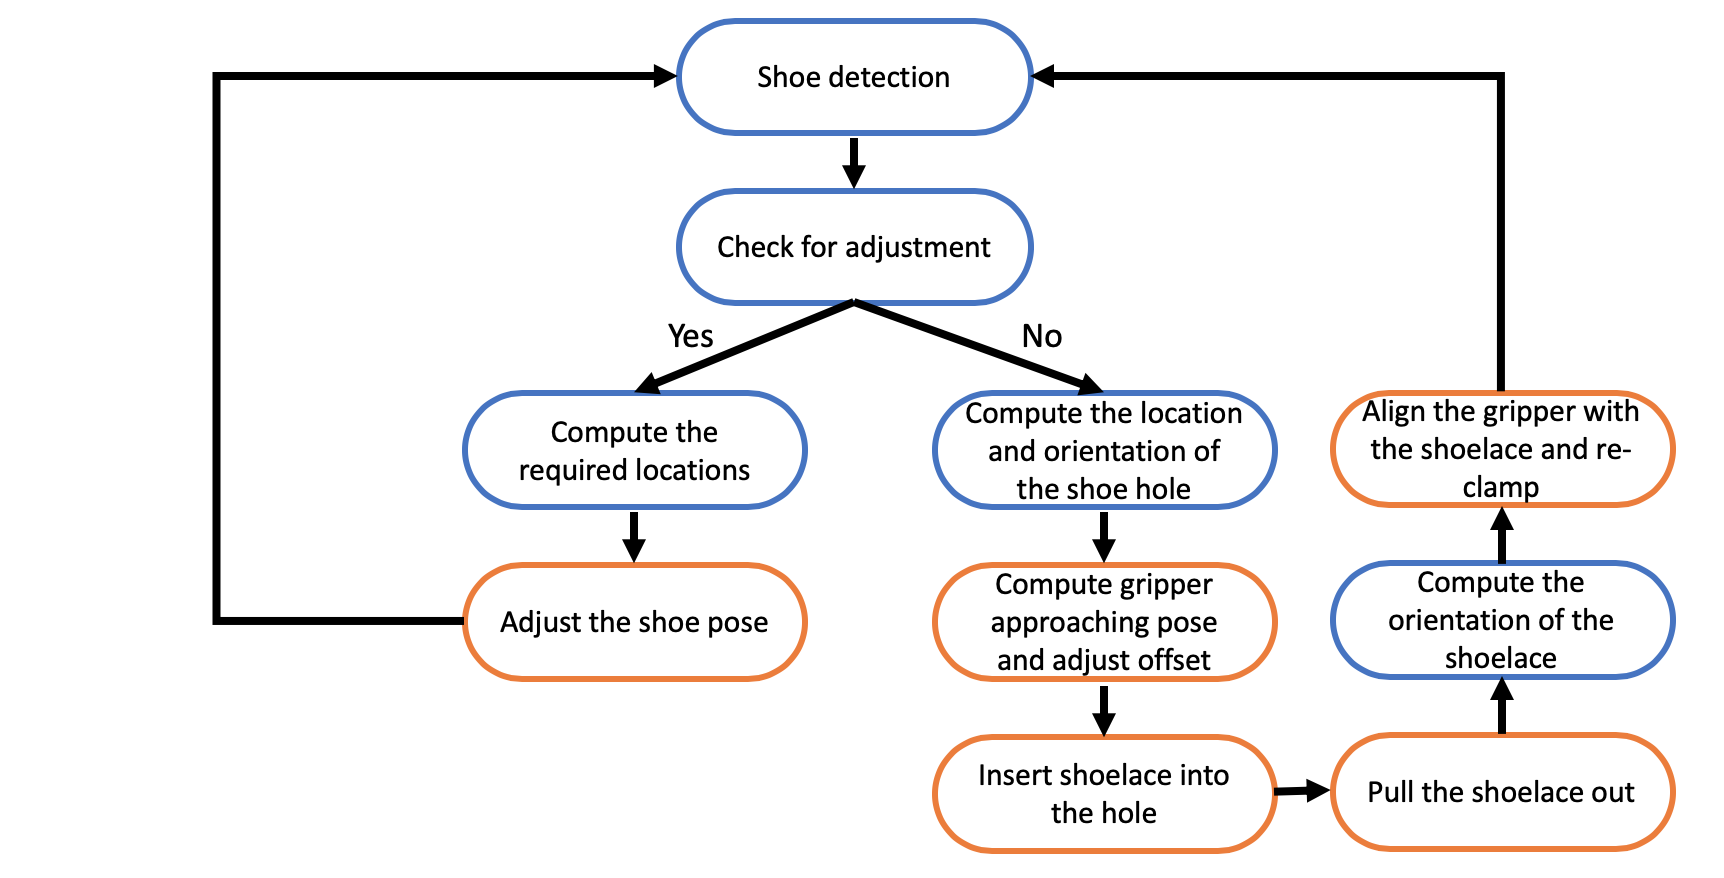
\includegraphics[width = \columnwidth]{AnalysisDesign/workflow.png}
\caption{System workflow for both core project and the extension}
\label{workflow}
\end{figure}

Figure \ref{workflow} is the illustration of the detailed algorithm workflow, where orange boxes are motion planning related and blue boxes are about computer vision. Starting with shoe detection, the system will then evaluate whether the shoe is in a good pose for manipulation or not. If the answer is negative, the required locations for adjustment will be computed and YuMi should manipulate the shoe accordingly. On the contrary, the system will calculate the gripper approaching pose for shoelace insertion based on the estimated 6D pose of the shoe hole. Once the offset is correctly adjusted, YuMi will pass the shoelace into that hole and pull it out. Finally, the 6D pose of the lace will be calculated, and the YuMi will reclamp it so that the gripper and shoelace can be aligned. After this stage, the system is back to shoe detection and ready for the next hole.

This workflow allows YuMi to plan a sequence of arm trajectories to put the shoelace on the shoe hole up to finishing the whole shoe. The following two chapters will discuss detailed implementation approaches for computer vision module and motion planning module, respectively.